\chapter{Presenting structured documents with {\Xprez}} \label{chap:presenting}



\bc
TODO:

empty and neutrality? stretching?

goed naar taaltje kijken, komen vast vragen over.

not urgent:
CHECK hansen function based formatting (Bib from Rui)
Check out  Yahu & wxHaskell for alternative ways of handling presentation attributes. Can these handle synthesized attrs as well?
\ec




%with this def:  \def\ch{chap:presenting}        we can use chapter specific labels like \label{\ch:labelname}






Although there are many presentation languages for structured documents (e.g.~\cite{css2, badros99ccss, marden98psl, xsl10, quint97thot}), not a single one seems to have sufficient expressiveness and abstraction mechanisms to specify the presentations of the use cases from Chapter~\ref{chap:requirements}. Pretty-printing libraries (e.g~\cite{oppen80prettyPrinting, swierstra98combinators, hughes1995prettyPrinting, kahl99galleyCombs, brand96generationOfFormatters}) do offer expressiveness, abstraction mechanisms, but these libraries are mainly text-oriented. 

In this section, we introduce the presentation language of Proxima: {\Xprez}. The language is an extended version of the presentation level that was discussed in Section~\ref{sect:presLevel}. {\Xprez}  has been implemented in Haskell. \bc It does not yet have a domain-specific syntax, but other than that it meets the requirements.\ec Although the language is not yet fully developed, it \bc is already powerful enough to describe a \TeX -like presentation with a style sheet of about 300 lines. \ec
 is already powerful enough to cover much of the \TeX~math typesetting as described in \cite{heckmann97functionalTex}. 
 
Below are two screenshots of example {\Xprez} presentations containing ligatures (e.g.\ the ``fi'' in ``Scientific'') and several mathematical constructs. An editor for these presentations can already be instantiated with the Proxima prototype, but in order to support pleasant editing, the prototype requires a few more extensions.

\begin{center}
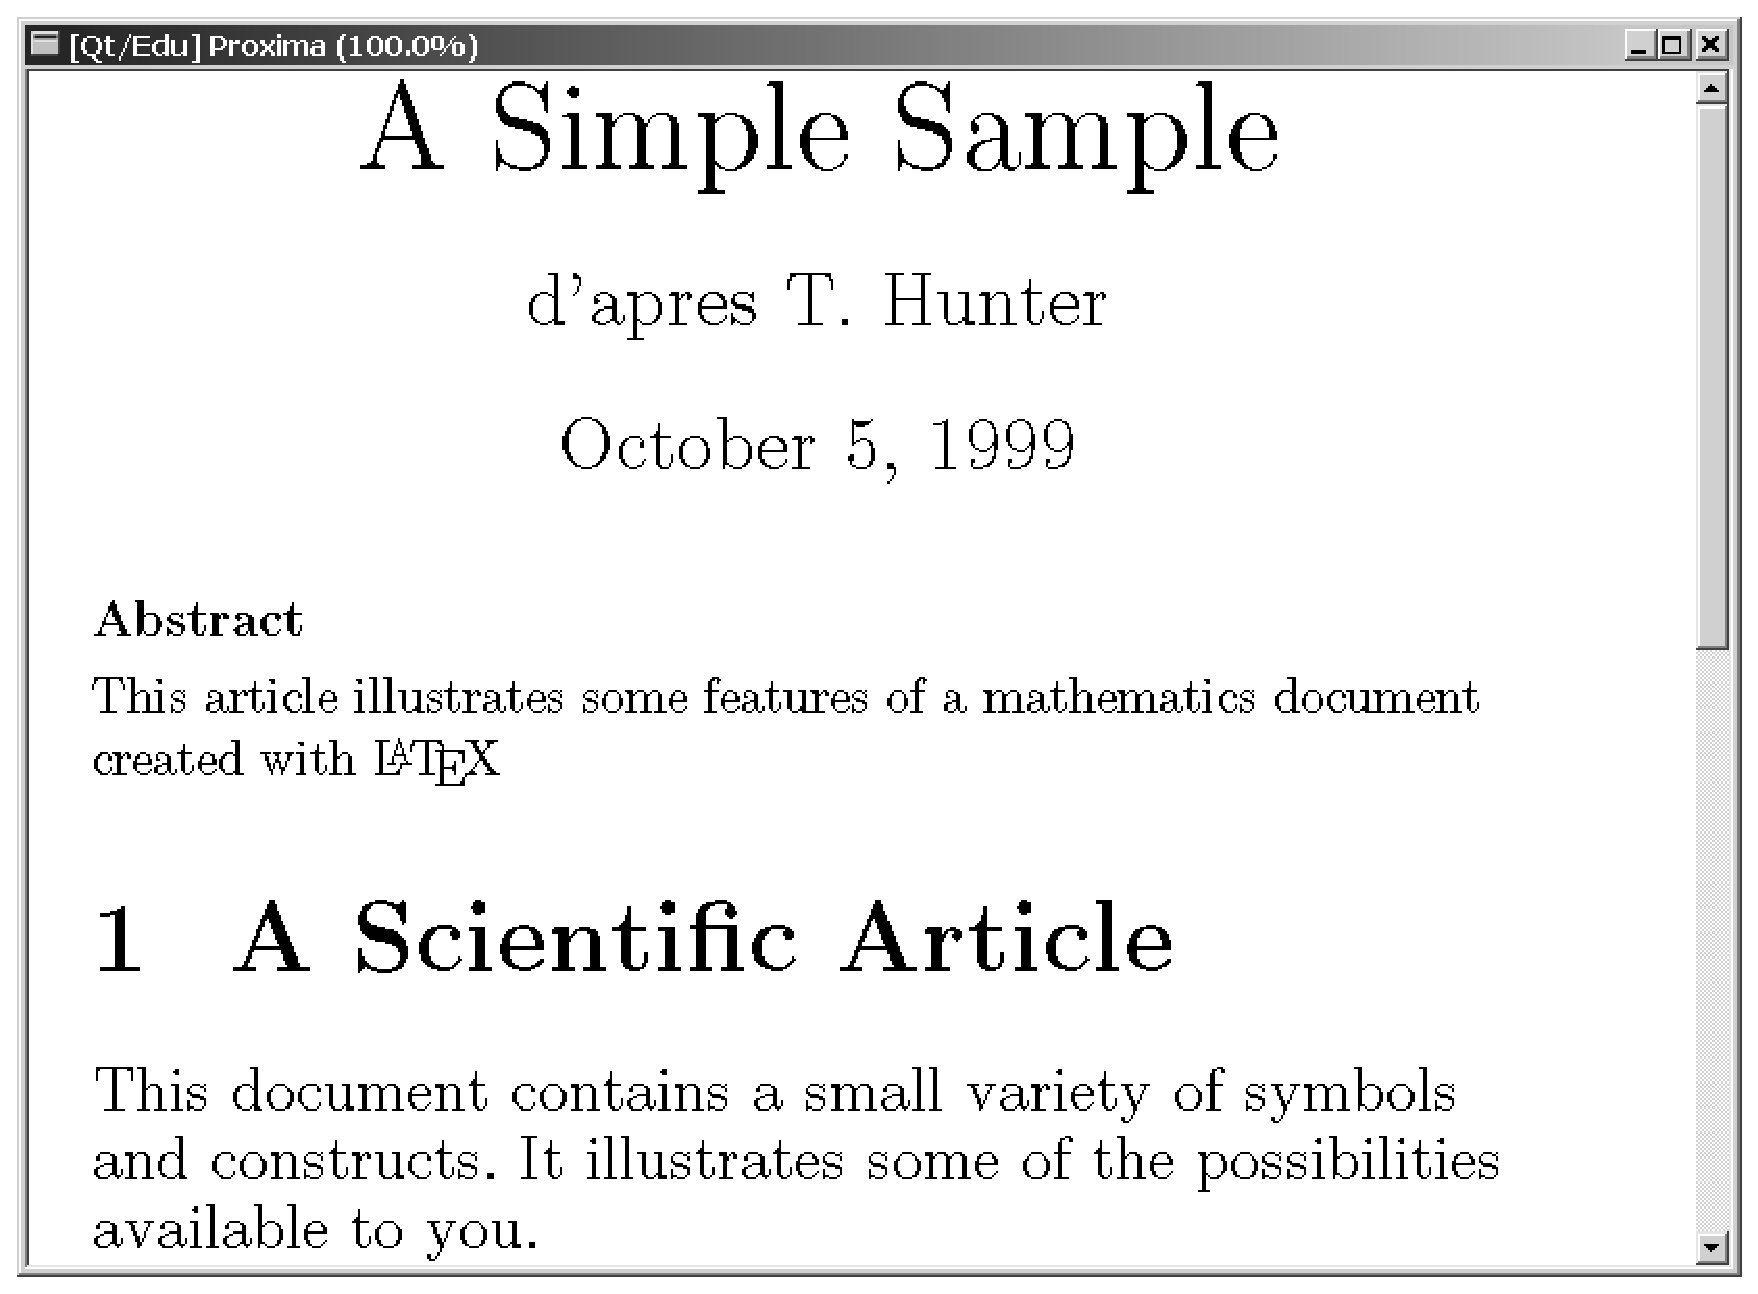
\epsfig{file=pics/eps/xlatex1.png.eps, width=1.9in} \qquad
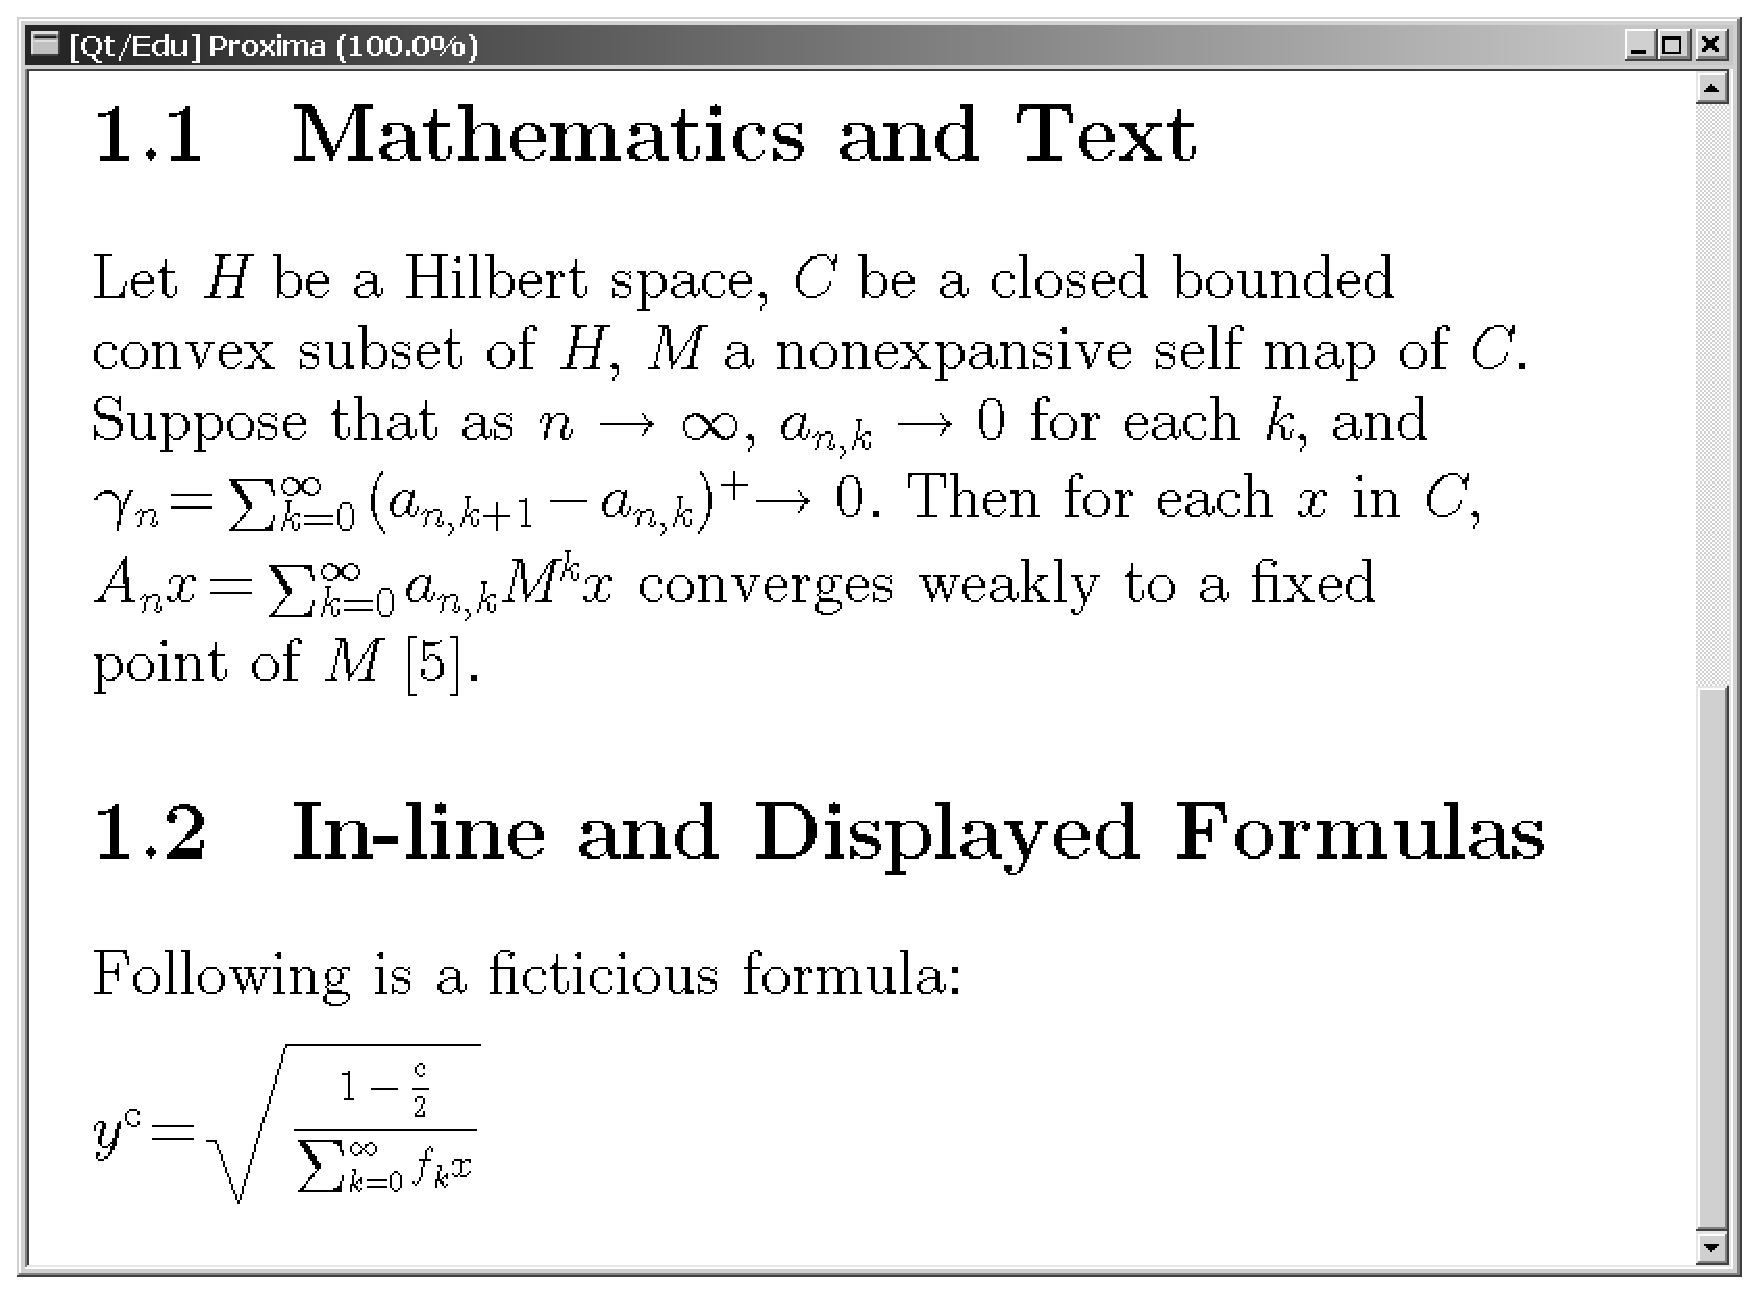
\epsfig{file=pics/eps/xlatex2.png.eps, width=1.9in}
\end{center}

%Contributions of this paper:

\bc
The contributions of this paper are:

\begin{itemize}
\item An evaluation of the strengths and weaknesses of existing presentation languages, resulting in a list of requirements for a presentation language.
\item A proposal for the declarative presentation language {\Xprez} that supports both the flow and the box model, has presentations as first-class objects, and has a powerful abstraction mechanism.
\end{itemize}
\ec

The {\Xprez} language consists of a set of Haskell combinators that can be used to define a presentation. A presentation is tree-structured and represents an attribute-grammar tree. The attributes are presentation attributes such as font size and color. A special combinator is available for modifying presentation attributes. 

Section~\ref{sect:targetlangs} discusses several existing presentation languages and states a number of requirements for a presentation language. This is followed by an informal description of the {\Xprez} presentation language in Section~\ref{sect:xpreztarget}. Section~\ref{sect:conclusions} concludes with an overview of future research.


%																
%																
%																
\section{Presentation languages} \label{sect:targetlangs}

In this section, we discuss five presentation languages for structured documents. XSL~\cite{xsl10} is a presentation language for XML documents, whereas CCSS~\cite{badros99ccss} and PSL~\cite{marden98psl} are presentation languages for HTML. CSS~2.0~\cite{css2} can be used to present both XML and HTML documents. Finally, the language P~\cite{quint97thot} is the presentation language of the Thot editor toolkit (see Section~\ref{sect:toolkits}). 

In Section~\ref{sect:presentationFormalism}, we mentioned that a presentation language consists of two parts. One part is the {\em presentation target language}, which describes the components (strings, boxes, rows, etc.) of a presentation. The other part is the {\em presentation specification language}, in which we specify how a document is mapped onto an element of the target language. Not every presentation language explicitly indentifies its presentation target language. Moreover, if the target language supports abstraction, a presentation may contain functions, which makes it difficult to clearly separate the two languages.

In the remainder of this chapter, we focus on presentation target language, because {\Xprez} is the presentation target language of Proxima. The presentation specification language of Proxima is an attribute-grammar formalism, but the details of this formalism still require further research. Section~\ref{sect:instantiating} provides more information on the presentation attribute grammar, as well as a few example presentation specifications. 

In most presentation languages, a presentation is a tree structure, in which the leaves are atomic presentations and the nodes are composite presentations. An atomic presentation is a string or a simple graphical objects such as a line, a box, or an image. On the other hand, a composite presentation specifies for a number of child presentations how these are put together. We distinguish three different layout models for composite presentations: a box, a matrix, and a flow layout.

\begin{description}
\item[Box layout]
In a box layout, child presentations are positioned relative to each other, for example horizontally in a row, or vertically in a column. The exact positioning may be specified for the entire list of children (e.g.\ by using a row or column combinator), or for each child itself, by specifying how it should be positioned relative to its sibling. A box model may provide facilities for aligning and stretching child presentations.

\bc The positions can be set either directly or relative to positions of other presentations, or by declaring constraints. If constraints are used, the style sheet does not so much specify the exact computation of a presentation attribute, but rather gives constraints that should hold for the attribute. The actual computation of the attribute value is left to a constraint solver. \ec
\item[Matrix layout]
A matrix model is similar to a box model, but aligns its children both horizontally and vertically. Because it is more general than a row or a column, a matrix may be used to create a box layout. 

\bc  be used to align a grid of elements, usually a list of rows that each contain a list of elements. The elements are aligned along the rows as well as the columns. This is difficult to specify just using rules for each row and cell, as the width of the n-th cell %has to be related to the n-th cells in the other rows instead of to properties \todo{properties?} of its parent or sibling cells.** 

Matrices can be used to create box presentations, but the extent to which this is possible depends on the expressivity of the matrix model; for example, whether or not cells may overlap.
\ec

\item[Flow layout]
 % does not depend on doc structure, but on available space. final presentation is not tree of target, but split 
 %along lines and pages

A flow layout is used for line- and page-breaking. Child presentations are placed next to or below each other, until the remaining space is too small to fit the next presentation, in which case a new line or page is started. Thus, unlike in a box or matix layout, the final structure of the presentation is only partially determined by the structure of the presentation.

% How the presentations are divided over the lines and pages depends on the size of the presentation
%
%Using a flow model, lists of words can be divided into lines and lists of lines can be divided into pages. The generated list of %flows may then be manipulated further, for example, by extending each page in a list of pages with a header and a footer.
\end{description}

Besides constructs for specifying the structure of the presentation, presentation languages also have a notion of presentation attributes (sometimes called properties). A presentation attribute affects the style, size, or position of a presentation, but not its structure. Examples of presentation attributes are font size, background color, alignment information, etc.


%																
\subsection{Existing presentation languages} \label{sect:existingtarget}

Of the five presentation languages we examined, only XSL regards its target language as a language in its own right, with a separate syntax. The other languages only describe how presentation attributes of the elements of the target presentation tree can be set, but do not treat a presentation as an actual value in the language.

\head{CSS~2.0:} Cascading Style Sheets, level~2~\cite{css2} is an example of a simple presentation language. Its target language is almost invisible to the style sheet designer.  \bc The presentation of a document is a tree that is almost isomorphic to the document tree, with the document content in the leaves. It is not entirely isomorphic, because content can be left out and simple text content can be added. \todo{flow} \ec A presentation is a tree structure, in which the nodes specify presentation attributes such as font size or color, and the leaves are document content. A presentation attribute may be specified either absolutely or as a percentage. In the latter case, the kind of the attribute determines what attribute the percentage refers to. For instance, a percentage value for the {\em font-size} attribute refers to the font size of the parent element, but a percentage for the {\em line-height} attribute refers to the font size of the element itself. It is not possible to let the value of a presentation attribute depend on arbitrary presentation attributes of the parent or siblings in the presentation tree.

CSS~2.0 supports a flow layout and a table format for a matrix layout. However, the control over alignment in the matrix model is rather weak.

\bc but it is of limited use because the transformation language is rather weak. Consequently, if the data in the document does not have exactly the same structure as a CSS~2.0 table, it cannot be presented as one.
\ec
\head{CCSS:} Constraint Cascading Style Sheets~\cite{badros99ccss} is an extension of the CSS~2.0 standard that is based on constraints. The target language of CCSS closely resembles the CSS~2.0 target language, but presentation attributes for a child are specified using constraints instead of percentages of the parent's attribute values. Another difference is that the constraints may refer to global constraint variables and to left-siblings in the presentation tree as well as to the parent node. Similar to CSS~2.0, CCSS supports a flow and matrix layout, but no box layout.

\head{XSL FO:} On the other side of the spectrum is the XSL stylesheet language for XML. The design of the target language, XSL Formatting Objects, was based on the flow objects of the DSSSL~\cite{dsssl96} presentation language for SGML. The formatting objects standard consists of a large collection of elements that can be used to specify page models, presentation attributes, and more complicated presentation aspects, such as hyphenation and counters. A presentation is a tree that consists of these formatting objects. 

XSL FO offers strong control over the flow model, but a box model is not supported. The matrix (table) model for XSL FO has more control over alignment than CSS~2.0, but horizontal alignment is still poorly supported. Hence, a mathematical formula cannot be displayed elegantly in XSL FO.

%but using it to create a box layout is difficult, because that requires the style sheet to take care of computing the alignment, 
%and XSLT does not support a strong computational formalism.

\head{PSL:} The Proteus Stylesheet Language~\cite{marden98psl} is an attempt to combine the simplicity of CSS~2.0 with the power of XSL. PSL extends the CSS target language with a box model and graphical symbols. The value of a presentation attribute (which is called a property in PSL) can be expressed as a mathematical expression that refers to presentation attributes of nodes in the presentation tree. This mechanism is called {\em property propagation}. 

PSL supports a flow model and a constraint-based box model, but lacks a matrix model. A presentation can specify its attributes for position and size relative to position and size attributes of other presentations in the tree. These other presentations can be addressed using a number of primitive functions for accessing siblings, parents, ancestors of a specific type, etc.

\head{P:} The  language P is the presentation language of the Thot editor toolkit~\cite{quint97thot}. It has a target language that consists entirely of boxes, which may be composed according to a box, a flow, or a matrix model. P supports horizontal and vertical reference lines for automatic alignment of boxes. Instead of having a large number of different presentation boxes, similar to XSL Formatting Objects, P has only three kinds of boxes with a large number of presentation attributes. In contrast to PSL, the box layout in P is not constraint-based. \bc Hence, the style sheet designer needs to take the order of computation of the layout properties** into account. \ec 

\head{Discussion:} 

The languages discussed above are all declarative and domain-specific languages that vary in expressive power. The languages CSS~2.0, CCSS, and PSL allow simple presentations to be specified in a simple way, but cannot be used to specify more complex presentations, such as mathematical formulas. In contrast, XSL and P allow complex presentations to be specified, but due to the lack of abstraction, simple presentations also have rather elaborate specifications, especially in P. 

Only P and PSL support a box model, but both models are of a rather object-oriented and imperative nature. Moreover, presentations are not first-class values. A box can specify its own position attributes relative to its parent or siblings, but it is not possible to state at parent-level that two child presentations should have their top and bottom aligned, or that two presentations should have the same width. \bc Thus, a conceptually simple change of presenting the children of a node next to each other instead of below each other requires changing the presentations for all child elements.\ec 

Letting a child presentation specify its own layout makes it more difficult to understand a presentation. For example, to reverse the presentation of a horizontal list of children, each child must specify that its right side must be aligned with the preceding child's left side. Moreover, if the the order of the children depends on an attribute of the parent, then the presentation definition of each child need to access this parent attribute and use its value to determine the alignment of the child.

If, on the other hand, child presentations are first-class, and abstraction mechanisms can be used to define combinators on them, a list of children may be reversed with a reverse function in the presentation definition of the parent.  Another advantage of this approach is that the concepts of layout direction (horizontal or vertical) and order of the children are orthogonal now. The layout direction is determined by which combinator is applied to the list of children, whereas the order is determined by whether or not a reverse function is applied to the list. In the model of P and PSL, these concepts are intertwined, and reversing a horizontal list is conceptually different from reversing a vertical list.

\head{ Requirements}

Based on the requirements from Chaper~\ref{chap:requirements} and the previous discussion, we conclude that the presentation target language for Proxima, should meet the following requirements: 

\begin{description}
\item[Proportional effort]
It must be possible to specify complex presentations, but the specification of simple presentations should still be easy.
\item[Declarative]
In a declarative language, understanding a composite presentation is easier, because the computation of a presentation does not generate side effects. Another advantage is that the designer need not worry about the order of computation of presentations and attributes.
\item[First-class presentations]
A first-class presentation can be named and manipulated at the level of its parent, which in many cases is the natural place for such manipulations. At the same time, it is also possible to specify aspects of the presentation at the level of the child when this is more appropriate.
\item[Box, matrix, and flow layout]
All four layout models mentioned at the start of this section should be supported. The alignment of the box and matrix models must be powerful enough to specify complex presentations such as mathematical formulas. 
\item[Text, graphical, and widgets]
It must be possible to specify text and graphical elements such as lines, boxes, and images. Moreover, the language must support user-interface widgets, such as buttons, selection lists, and menus. 
\item[Powerful abstraction mechanism]
User-defined functions and variables help to reduce code duplication, facilitate code reuse, and increase transparency, because complex pieces of code may be replaced by functions with well-chosen names.
\item[Domain-specific]
The language should have syntax for presentation-specific constructs such as an {\bf ex} (the height of the letter `x' in the current font and size) and different measuring units such as pixels and inches.
\end{description}
\bc
\begin{itemize}
\item Complicated presentations should be possible, but at the same time simple presentations should be easy to specify.
\item The language should be declarative. Thus, the order in which presentation rules are specified is not important.
\item Domain-specific syntax should be available for presentation-specific constructs. 
\item It should support a flow (\`a la XSL) and a box (\`a la \TeX) model with alignment.
\item Presentations should be first-class values. Thus presentations can be manipulated, passed as arguments to functions, etc.
\item It should have a powerful abstraction mechanism. Thus, similar presentations can be specified with one, appropriately parameterized, function.
\end{itemize}
\ec



%																
%																
%																
\section{The {\Xprez} target language} \label{sect:xpreztarget}

With the requirements from the previous subsection in mind, we have developed the declarative presentation language {\Xprez}. 

%																
\subsection{{\Xprez} presentation model}

Similar to P and the document formatting languages \TeX ~and Lout~\cite{kingston93lout}, {\Xprez} is a box language with support for flow layout. A presentation is a value of the abstract type \p{Xprez}, and is either an atomic box containing a text or a graphical object, or a composite box that contains a list of child presentation boxes.  We construct \p{Xprez} values in the functional language Haskell, using a number of primitive functions that are described in Section~\ref{sect:primitives}.

\begin{figure}
\begin{small}
\begin{center}
\begin{small}
\begin{verbatim}
data Inh = Inh { fontFamily :: String, fontSize :: Int,
                 textColor, lineColor, fillColor, bgColor :: Color } 
data Syn = Syn { hRef, vRef, minWidth, minHeight :: Int,
                 hStretch, vStretch :: Bool}
\end{verbatim}
\end{small}
\caption{The {\Xprez} presentation attributes}\label{xprezattributes} 
\end{center}
\end{small}
\end{figure}


A presentation box (from now on called presentation) has a number of attributes that describe its size and its appearance: 

\begin{center}
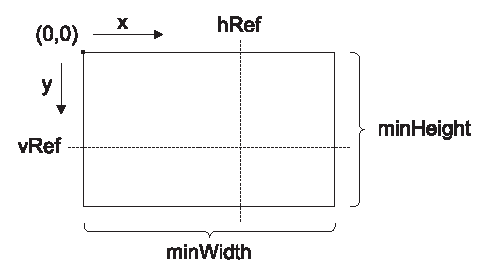
\epsfig{file=pics/eps/PresentationBox.eps, width=2in}
\end{center}

A presentation tree in {Xprez} represents an attribute grammar with inherited and synthesized attributes. Presentation attributes that are typically specified for an entire subpresentation, such as color and font size, are inherited attributes  \bc (going downward in the tree)\ec. On the other hand, presentation attributes that are set by a child and used by its parent, such as  reference lines and size information, are synthesized attributes. Figure~\ref{xprezattributes} shows the two Haskell records  \p{Inh} and \p{Syn} that are used to model the inherited and synthesized presentation attributes. The figure also shows the type of each attribute. 

The \p{hRef} and \p{vRef} attributes specify the horizontal and vertical reference lines that are used for aligning boxes when combined in composite presentations. Note that the vertical reference line is in fact a horizontal line and vice versa. The term vertical reference line stems from the fact that it is used for vertical alignment; modifying the vertical reference line affects the vertical position of the presentation. 

The boolean \p{hStretch} and \p{vStretch} specify whether or not the presentation is allowed to stretch in horizontal or vertical direction. The remaining attributes are the self-explanatory: \p{fontFamily}, \p{fontSize}, \p{textColor}, \p{lineColor}, \p{fillColor}, and \p{bgColor}. In the future, this set will be extended with other attributes such as line and font style, and attributes for modeling edit behavior (e.g.\ \p{onMouseClick~::~EditCommand}). \bc and user-defined attributes will be supported. \ec

\bc
The presentation tree is transformed into an attribute grammar in which the font, style, and color properties are inherited attributes that go down in the tree, and alignment and stretch properties are synthesized attributes that go up in the tree. In the Haskell types, this division is visible in the fact that the properties are modeled using two records: \p{Inh} for inherited properties, and \p{Syn} for synthesized properties.
\ec

%																
\subsection{{\Xprez} primitives} \label{sect:primitives}

The first five combinators in Figure~\ref{xprezprim} specify atomic presentations. The \p{empty} combinator is not visible and takes up no space, it is the neutral element for composite presentations. A string is presented with \p{text}, and a rectangle with \p{rect}. The \p{poly} combinator takes a list of relative coordinates between (0.0, 0.0) and (1.0, 1.0) and produces a line figure that connects these points. The coordinates are relative because the final coordinates depend on the size of the \p{poly} presentation. Finally, \p{img} can be used to display external images. The argument is a string that contains the path to the image file. In a future version, an \p{img} may also contain a reference to an image that is encoded as part of the document.

Except for \p{text}, the horizontal and vertical reference lines of an atomic presentation are both 0 (i.e.\ the north-west corner). For \p{text},  the vertical reference line is the baseline of the text and the horizontal reference line is 0. By default, a  simple presentation does not stretch.

\begin{figure}
\begin{small}
\begin{center}
\begin{small}
\begin{verbatim}
empty             :: Xprez
text              :: String -> Xprez             
rect              :: Xprez                       
img               :: String -> Xprez             
poly              :: [ (Float, Float) ] -> Xprez 
row, col, overlay :: [ Xprez ] -> Xprez          
rowR, colR        :: Int -> [ Xprez ] -> Xprez   
matrix            :: [[ Xprez ]] -> Xprez
format            :: [ Xprez ] -> Xprez
\end{verbatim}
\end{small}
\caption{The {\Xprez} primitives} \label{xprezprim} 
\end{center}
\end{small}
\end{figure}

%-- simple text           
%-- rectangle             
%-- image (jpg, png, ...) 
%-- poly line             
%-- row, column, overlay  
%-- row, col w/ reference 

The remaining primitives in Figure~\ref{xprezprim} specify composite presentations. The behavior of columns (\p{col}) is equal to that of rows (\p{row}) with the horizontal and vertical directions swapped. Hence, we only discuss the \p{row} primitive. In a row, each child presentation is placed immediately to the right of its predecessor, with their vertical reference lines aligned. Horizontal reference lines have no effect on the positioning in a row.

\begin{center}
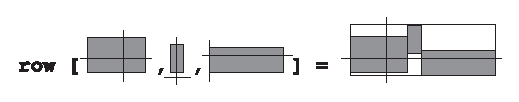
\epsfig{file=pics/eps/row.eps, width=3.2in}
\end{center}

The bounding box of a row is the smallest rectangle that encloses all elements of the row. The vertical reference line of the row is equal to the aligned reference lines of the children, whereas the horizontal reference line is taken from the first child. In order to use the horizontal reference line from one of the other children, we can use the \p{rowR} combinator. The integer argument of \p{rowR} specifies which child determines the horizontal reference line for the row, with 0 denoting the first child. 

By default, a row stretches in horizontal direction if one of its children does, and it stretches in vertical direction if all children stretch vertically. The defaults may be overridden by setting the stretch attributes with the method that is  shown in the next section. 

The \p{matrix} combinator can be used to describe a table layout, in which elements are aligned with elements to their left and right as well as with elements above and below them. 

Because \p{row}, \p{column} and \p{matrix} do not allow their children to overlap, we need a special combinator for overlapping presentations. The \p{overlay} combinator places its children in front of each other, while aligning both the horizontal and vertical reference lines. It can be used to create underlined text, for example. Because alignment takes place on both reference lines and hence all child reference lines overlap, no special \p{overlayR} combinator is needed.

A flow layout can be achieved with the \p{format} combinator for paragraph formatting. The combinator takes a list of presentations as argument and splits this list into rows based on the available horizontal space. The resulting rows are placed in a column.  Because \p{Xprez} does not yet have a page model, only horizontal formatting is supported. 

Here is an example {\Xprez} presentation that illustrates alignment and stretching in a row:

\begin{small}
\begin{verbatim}
let cross     = poly [(0,0),(1,0),(1,1),(0,1),(0,0),(1,1),(0,1),(1,0)]
    greycross = cross `withbgColor` grey `withStretch` True
in  row [ text "Big" `withFontSize` 200
        , colR 2 [ cross, cross, text "small", greycross, greycross ] ] 
\end{verbatim}
\end{small}

The code produces the following image (the dashed line has been added to show vertical reference line of the presentation):

\begin{center}

\epsfig{file=pics/eps/align.png.eps, width=1in}
\end{center}

The second element in the row is a column that takes the vertical reference line from its third child. Therefore, the word ``Big'' is aligned with the word ``small''. The \p{cross} object is a line figure in the form of a rectangle with a cross, which is made stretchable in both directions by \p{withStretch}. The \p{greycross} is a \p{cross} with a grey background. 
 
Because the column contains presentations that stretch vertically, the column itself also stretches vertically. The two stretching objects above the reference object (\p{text "small"}) are each assigned equal amounts of the remaining space above the vertical reference line, and likewise, the objects underneath the reference object are assigned the remaining space below the reference line. If, on the other hand, the reference object itself is allowed to stretch, then the total amount of available space is distributed equally over all stretching objects. In this case, the reference object is not aligned. 

%																
\subsection{Modifying presentation attributes}

The presentation attributes of a presentation can be modified using the \p{with\symbol{95}} combinator (The name gets an underscore because the keyword \p{with} is already defined in Haskell).

\begin{small}
\begin{verbatim}
with_ :: Xprez -> ((Inh, Syn) -> (Inh, Syn)) -> Xprez
\end{verbatim}
\end{small}

The combinator takes a single child presentation as argument, together with a function from attributes to attributes. The function is applied to the inherited attributes coming from the parent, and the synthesized attributes coming from the child. From the result of this application, the inherited attributes are passed to the child, whereas the synthesized attributes are passed to the parent. Thus, the \p{with\symbol{95}} combinator can be used to modify the inherited and synthesized attributes of a presentation.

\begin{figure}[t]
\begin{center}
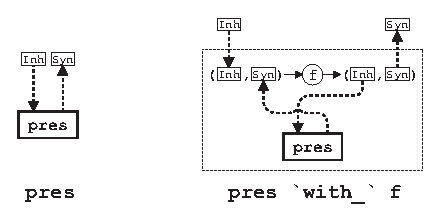
\epsfig{file=pics/eps/with.eps, width=6cm} % visio: With.vsd
\caption{Data flow for \p{with\symbol{95}}.}\label{withDataFlow} 
\end{center}
\end{figure}


Figure shows the data flow for the attributes of \p{pres} and \p{pres `with\symbol{95}` f}. At the top-right of the figure, \p{Inh} and \p{Syn} are swapped to prevent crossing arrows. Because \p{f} may be an arbitrary function, the combinator may introduce cycles in the attribution. It is up to the designer of the presentation to ensure safety.

\bc \toHere
In the specification of an attribute value, the original values of attributes can be used (e.g.\ the font size can be set to the old font size increased with 2 points). Therefore, the second argument of \p{with\symbol{95}} is a function that %takes as arguments the inherited attributes coming from the parent and the synthesized attributes coming from the %child presentation as arguments, and returns the new values (i.e.\ the inherited attributes that go to the child and the synthesized attributes that go to the parent).
\fromHere \ec

Because the inherited and synthesized attributes are modeled as Haskell records, we use the Haskell record syntax for  accessing and updating presentation attribute values. Hence, for a record of inherited attributes \p{inh :: Inh}, the expression \p{fontSize inh} denotes the value of the \p{fontSize} attribute in \p{inh}. Furthermore, \p{inh $\{$ fontSize = 10 $\}$} denotes a copy of \p{inh} in which the \p{fontSize} field is updated to 10. Thus, we can define a  \p{withFontSize} combinator: 

\begin{small}
\begin{verbatim}
withFontSize :: Xprez -> Int -> Xprez
withFontSize xp fs = xp `with_` \(inh, syn) -> (inh {fontSize = fs}, syn)
\end{verbatim}
\end{small}

The function argument to \p{with\symbol{95}} introduces a considerable syntactic overhead to the presentation code. To reduce this overhead, we can define a library of combinators, such as \p{withFontSize}, for frequent applications of  \p{with\symbol{95}}. Thus, most of the explicit applications of \p{with\symbol{95}} may be avoided.

Besides combinators that set an attribute value absolutely, we can also define combinators that take into account the original value of an attribute when setting its value. Consider the combinator \p{withFontSize\symbol{95}} defined below. Instead of an integer, it takes a function (\p{ffs~::~Int~->~Int}) as argument. Given the inherited font size, the function \p{ffs} specifies its new value.

\begin{small}
\begin{verbatim}
withFontSize_ :: Xprez -> (Int -> Int) -> Xprez
withFontSize_ xp ffs = 
  xp `with_` \(inh, syn) -> (inh { fontSize = ffs (fontSize inh) }, syn)
\end{verbatim}
\end{small}

With \p{pres `withFontSize\symbol{95}` (\symbol{92}fs -> 2*fs)} we specify that \p{pres} gets a doubled font size. An application of \p{withFontSize\symbol{95}} has a function argument, but the function is considerably simpler than for \p{with\symbol{95}}. 

\bc A more natural solution is the declaration of a special data type \p{Length}, with operations such as addition and multiplication, but which also has primitive values that represent current font properties***. In Haskell, type classes can be used to accomplish this. Using type classes, it will be possible to write: \p{vSpace (2*ex)}, which denotes a horizontal space of twice the height of the letter x in the current font.\ec 


The font-size combinators show how abstraction is used to meet the {\em proportional effort} requirement. For simple changes of the font size, the simple \p{withFontSize} combinator can be used, and only if more control is desired, it is necessary to use the more complicated \p{withFontSize\symbol{95}} or \p{with\symbol{95}} combinators.

A future version of {\Xprez} will support a domain-specific special syntax for \p{with\symbol{95}}. Thus, in order to specify that  a presentation \p{pres} gets twice the font size of its parent, a red background color, and a height that is twice the height of the letter `x' in the current font, we will be able to write something in the line of: 

\begin{small}
\p{pres\{ child.fontSize = 2*parent.fontSize, child.color = red, height = 1ex \}}
\end{small}

%																
\subsection{Advanced examples} \label{sect:xprezFrac}

Because a presentation in {\Xprez} is a first-class value, it is possible manipulate a child presentation (e.g.\ change its position or modify the font size) at the level of its parent.  This is illustrated in the presentation for a mathematical fraction: 

\begin{small}
\begin{verbatim}
frac e1 e2 = let numerator   = hAlignCenter (pad (shrink e1) )
                 bar         = hLine
                 denominator = hAlignCenter (pad (shrink e2) )
             in  colR 2 [ numerator, vSpace 2, bar
                        , vSpace 2, denominator ] `withHStretch` False

pad xp = row [ hSpace 2, xp, hSpace 2 ]

shrink e = e `withFontSize_` (\fs -> (70 `percent` fs) `max` 10)
\end{verbatim}
\end{small}

The non-primitive library function \p{hAlignCenter} centers its argument horizontally, and the \p{shrink} function reduces the font size to 70\%
, with a minimum of 10. The result of \p{(text "x" `frac` text "2") `frac` text "1 + y"} is:

\begin{center}
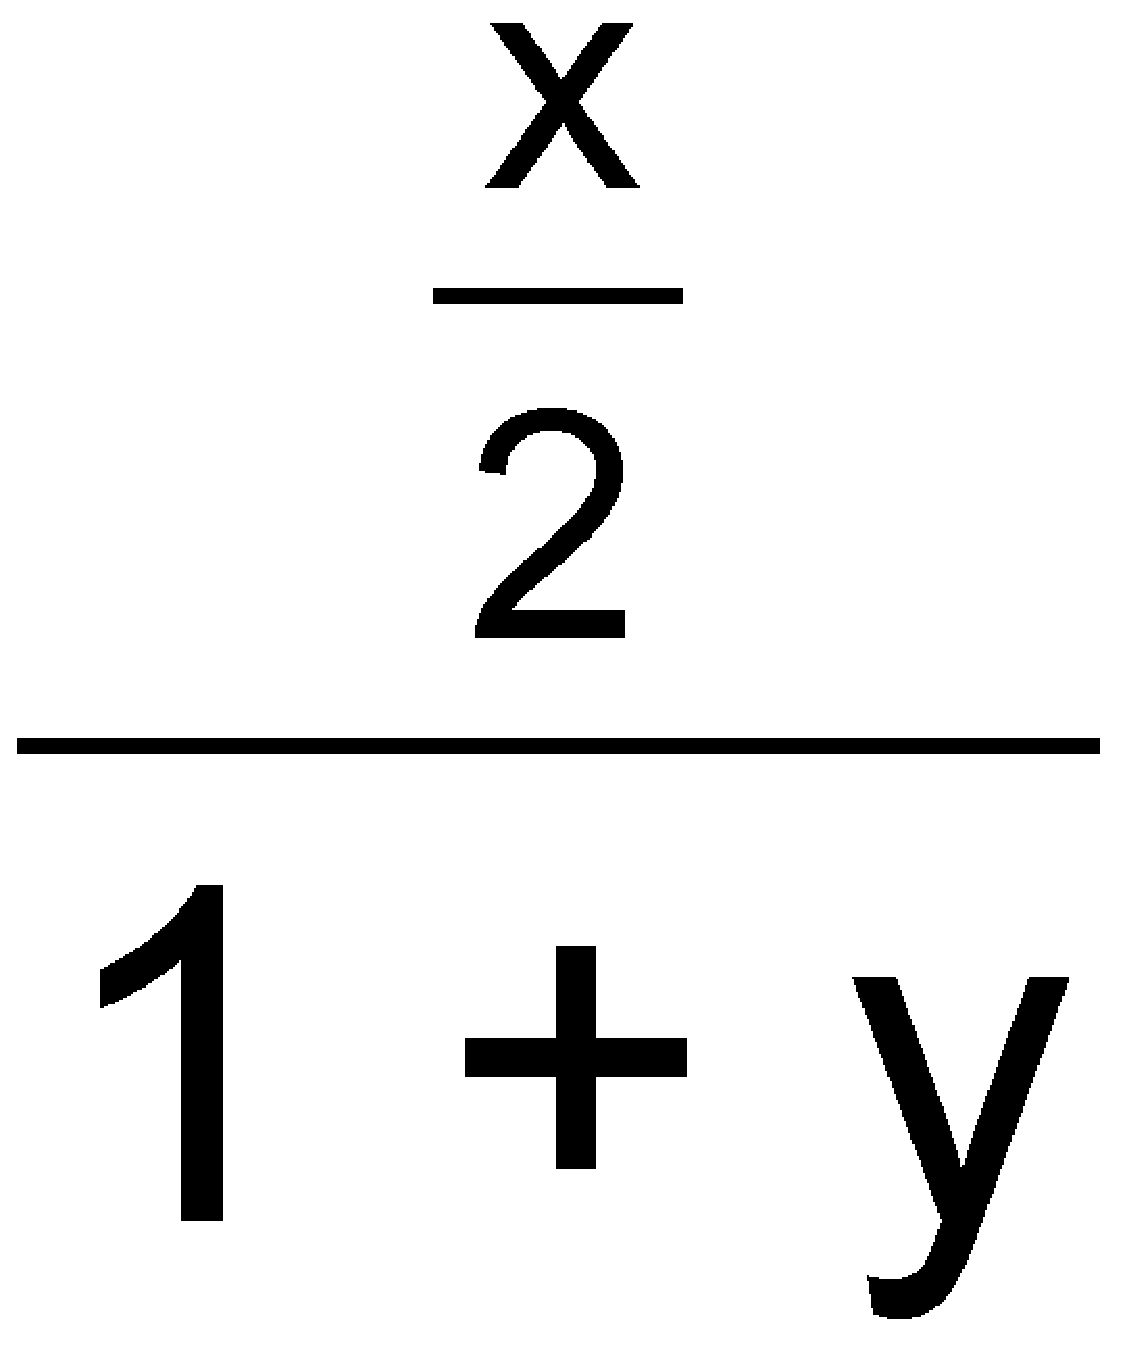
\epsfig{file=pics/eps/frac.png.eps, width=0.5in}
\end{center}

The \p{pad} and \p{shrink} functions illustrate the {\em first-class} and {\em abstraction} requirements. Because a presentation is a first-class value, the presentations of the numerator and the denominator can be resized and positioned in the presentation of the fraction itself. Furthermore, we can abstract over positioning and resizing by using the functions \p{pad} and \p{shrink}. 

In contrast, child presentations in both P or PSL cannot be addressed at parent level. Hence, the numerator, the denominator, and even the fraction bar, each have to specify their own size and relative position. As a result, it is difficult to reuse parts of a presentation in another presentation, since all parts refer to each other. Furthermore,  the manipulations on the appearance are harder to read, because no abstraction can be used. 


The second example is a pair of combinators that can be used to create tree-browser presentations:

\begin{center}
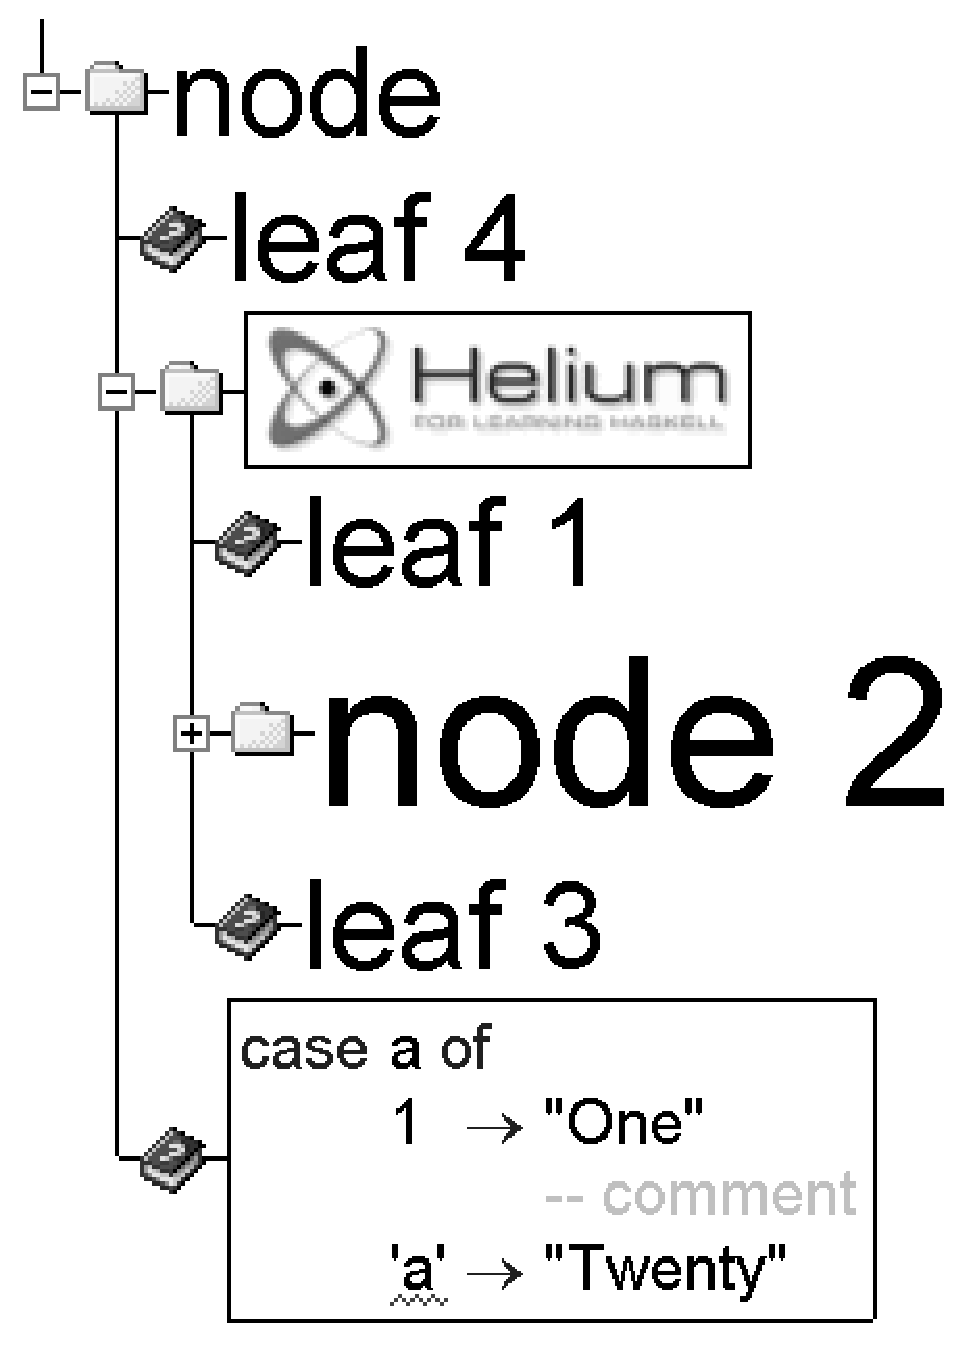
\epsfig{file=pics/eps/tree.png.eps, width=1in}
\end{center}


The image has been created with the \p{mkTreeLeaf} and \p{mkTreeNode} combinators, shown in Figure~\ref{treeCombinators}. Both combinators take an \p{Xprez} argument that is the presentation of the label, and the tree node also takes a list of child presentations (which should be either nodes or leaves for a correct tree). A label is not restricted to text, but can be an arbitrary {\Xprez} presentation, as shown by the case statement at the bottom of the tree. The tree example shows that a complex and graphical presentation can be specified with relatively little effort.

\bc However, in order to make this presentation a fully operational tree browser that can react to mouse clicks, we need to model the presentation state and edit operations on this state. This is not possible in the current version of {\Xprez} but will be possible in the Proxima editor system.
\ec

\begin{figure}[t] % float placement, see http://www.maths.uwa.edu.au/computing/software/tex/doc/FAQ.html
\begin{small}
\begin{center}
\begin{footnotesize}
\begin{verbatim}
mkTreeLeaf :: Bool -> Xprez -> Xprez
mkTreeLeaf isLast label = 
  row [ leafHandle isLast, hLine `withWidth` 5, leafImg
      , hLine `withWidth` 5, refHalf label ] 

mkTreeNode :: Bool -> Bool -> Xprez -> [Xprez] -> Xprez
mkTreeNode isExp isLast label children =
  rowR 1 [ hSpace 4, nodeHandle isExp isLast, hLine `withWidth` 5
         , col $ [ row [ col [nodeImg , if isExp then vLine else empty]
                       , hLine `withWidth` 5, refHalf label ] ]
                 ++ (if isExp then children else [] ) ]

nodeHandle isExp isLast 
 = colR 1 ([ vLine, handleImg isExp]++ if isLast then [] else [vLine])

leafHandle isLast = colR 1 ([vLine, empty]++ if isLast then [] else [vLine])

handleImg isExp = if isExp then minusImg else plusImg

nodeImg = img "folder.bmp" `withRef` (7,7)
leafImg = img "help.bmp"   `withRef` (7,6)
plusImg = img "plus.bmp"   `withRef` (4,4)
minusImg = img "minus.bmp" `withRef` (4,4)
\end{verbatim}
\end{footnotesize}
\caption{{\Xprez} tree-browser combinators}\label{treeCombinators} 
\end{center}
\end{small}
\end{figure}


%																
\section{Conclusions and further research}  \label{sect:conclusions}

Current style sheet languages lack either the expressiveness or the abstraction mechanisms to specify complex presentations in a readable way. The declarative presentation language {\Xprez}, introduced in this chapter, combines a flow and box model with a powerful abstraction mechanism and first-class presentations. The language is well-suited for specifying a wide range of presentations, from tree browsers to WYSIWYG presentations of mathematical formulas, using concise and readable presentation code. An implementation of {\Xprez} is part of the Proxima prototype. 

\bc The set of combinators we have presented is powerful enough to cover much of the \TeX~math typesetting as described in \cite{heckmann97functionalTex} \ec

{\Xprez} can already describe a large variety of presentations, but the language does not yet meet all the requirements of  Section~\ref{sect:existingtarget}. The language still needs a page model (required for vertical flow layout), support for user-interface widgets, and a domain-specific syntax.

%A page model for {\Xprez} also has consequences for the edit model of Proxima, since 
Once {\Xprez} has a page model and vertical flow layout, it will be possible to support page related concepts such as footnotes and page references. In order to support such presentations, an abstraction similar to the {\em galley} of Lout~\cite{kingston93lout} may be added to {\Xprez}.

In a flow layout, spacing between two presentations should be visible when they end up on the same line or page, but not when there is a line or page break between them. Hence, {\Xprez} needs a primitive notion of padding and margins for a presentation, which can be left out when appropriate. Moreover, the horizontal and vertical formatting algorithms need support for optimal line- and page-breaking~\cite{knuth82breaking}. To support formatting during editing, we could use either a linear algorithm (e.g.\ \cite{demoor99breaking}), or even an incremental algorithm (e.g.\ \cite{jeuring91breaking}).

Although support for primitive user-interface widgets to {\Xprez} will not have a large impact on the language, it is closely linked to the Proxima edit model. Hence, more experience with building editors in Proxima is needed in order to establish the right model.

Finally, a domain-specific syntax may be supported using the mechanism of syntax macros~\cite{leavenworth66synMacros}, for which a Haskell implementation has been developed. Until a domain-specific syntax is available, the syntax required for attribute modification may be reduced by using techniques similar to the property specification method of wxHaskell~\cite{leijen04wxHaskell}.

\bc A domain-specific syntax may be supported by using a syntax macro . Until a .. is available, the syntax of attribute specifications may be .. by using the property specification method of wxHaskell.
\ec

\bc
\cite{leijen04wxHaskell}
Syntax macro's - maybe intermediate sol. for syntax is properties as wxHaskell.
\ec


\bc Secondly, there is no primitive notion of padding, which will allow spacing in columns and rows to be specified more naturally. Both of these concepts are related to the need for a more powerful \p{format} primitive that can handle both horizontal and vertical formatting while offering more control over the generated rows and columns. 
\ec

In {\Xprez}  expressiveness and efficient evaluation are considered to be more important than safety. An {\Xprez} value is translated to an attribute grammar, in which the attribution may be influenced directly using the  \p{with\symbol{95}} combinator. This results in an expressive presentation language that can be efficiently evaluated, but also makes it possile to define presentations that crash, or cause cycles in the attribution.  A more restricted presentation language may guarantee safety, but will not be able to specify the complex presentations from Chapter~\ref{chap:requirements}. Hence, such editors need to be built by hand, which makes it considerably harder to guarantee safety.

%Of course better to have, but when confronted with weak pres lang building custom editor is unsafer. Nevertheless, conditions %on app of with. 

It will be interesting to see whether {\Xprez} can be integrated with a constraint solver. Constraints provide an elegant way to specify presentations, and also offer more safety . An entirely constraint-based version of {\Xprez}, which made use of the Cassowary linear constraint solving algorithm~\cite{badros01cassowary}, turned out too slow to be suitable for editing. However, it may be an option to use  a combination of the two formalisms (AG and constraints) in which constraints are used only for certain subpresentations, while attribute grammars are used for the remaining layout.

Besides extensions to the {\Xprez} formalism, an extensive library of well-chosen combinators must be established to facilitate the specification of complex presentations. And finally, it is desirable to have an algebraic model for {\Xprez} presentations. With such a model, we can describe the  exact behavior of the combinators with laws, rather than textual descriptions.



\bc
A Haskell implementation has been developed for both the target and transformation parts of {\Xprez}. It has been used to generate all screen shots in this paper. The user interface of this implementation is still in a premature stage, and the dependency on a number of different tools make it difficult to install. However, these are minor problems which require a fair amount of programming, but pose no major theoretical difficulties. 
\ec

% obsolete
\bc Finally, the \p{with\symbol{95}} combinator only gives access to the attributes of a parent and its child. It is not possible to access attributes of siblings, or presentations elsewhere in the tree, but it is also not yet clear whether such access is really necessary in a presentation language. 
\ec

\bc
Referee comments: 
The PADL 2002 Program Committee: PADL 2002 Decision,  Fri, 12 Oct 2001 15:27:12 -0400 (EDT) 
Harald Sondergaard: Your PPDP01 paper #16,  Mon, 7 May 2001 19:51:05 +1000 (EST) 
\ec









